% !TeX spellcheck = en_US
% !TeX root = ../BachelorThesis.tex

\section{2MWT} \label{section: 2MWT}
We want to investigate if the distance walked during the experiments of the 2MWT could say anything about the quality of the next day. 
Before we can actually use the results of the 2MWT, we must research how accurate and reliable the GPS on mobile phones is.
In Android, there is a method that can give us the accuracy of the retrieved location in meters \cite{androidaccuracy}.
However, this accuracy is only concerned with horizontal accuracy.
Bearing, velocity or altitude are not included.
The GPS is operational under all weather conditions\cite{bar2009geodetic} .
Weather conditions do not influence the accuracy of the position \cite{gpsweather}.
Obstructions like roofs and walls do block GPS signals.
The app should notify the user when the estimated error becomes too big.

Because the earth is not flat, there are actually no straight lines between two GPS coordinates.
To address this problem, there exist several algorithms to calculate the distance between two GPS coordinates.
%
\begin{itemize}
	\item The great-circle distance \cite{weisstein2002great} assumes that the earth is a sphere and uses the spherical law of cosines formula.
	
	\item The haversine formula can also be used to give great-circle distances between two GPS coordinates.
	This formula is better for small distances, because the formula is not too sensitive for a change of input.
	
	\item Methods based on the great-circle distance are less accurate than Vincenty's formula, which assumes that the earth is an oblate spheroid.
	This formula can be accurate up to the millimeter.
\end{itemize}
%
The error in the great-circle distance can be up to 0.5\%, which will result in an error of several centimeters in this case. 
Because the impact of this error is so low, we decided to use the great-circle distance instead.

To get more insight into the accuracy of the measured distance walked, two experiments were designed to test the inter device reliability and accuracy of calculated distance walked in the 2MWT using the `Mijn Kwik' app.
This is the same app that is used by the participants in our study.

\subsection{Experiment 1}

\subsubsection{Method}
In this experiment, we used the straight 100 meters on an all-weather running track as a comparison. The GPS coordinates, used for calculating the total distance walked, are registered at specific time intervals.
These intervals depend on the GPS signal and the used chipset. 
In this case, the time between the registration of consecutive GPS signals was between 4000 and 6000 milliseconds.
To calculate the distance walked, we first used linear interpolation to create a roughly smoothed line through the GPS coordinates.
Afterwards, a Savgol (Savitzky-Golay) filter \cite{press1990savitzky} was used to smooth this raw line. 
The coordinates returned by this Savgol filter where then used used to calculate the distance walked using the great-circle distance.

\subsubsection{Results and Conclusion}
%
\begin{table}
	\centering
	%
	\begin{tabular}{@{}lll@{}}
		\toprule
		\textbf{Device} & \textbf{OS}  & \textbf{GPS support} \\ \midrule
		Samsung Galaxy S3 Neo GT-I9301I (1) & 4.4.2 & A-GPS, GLONASS \\
		LG Leon (H320) & 5.0.1 & A-GPS\\
		Samsung Galaxy S3 Neo GT-I9301I (2) & 4.4.2 & A-GPS, GLONASS\\ \bottomrule
	\end{tabular}
	%
	\captionof{table}{Devices used in the experiment.}
	\label{2MWT: exp1 specs}
\end{table}
%
\begin{table}
	\centering
	%
	\resizebox{\textwidth}{!}{
	\begin{tabular}{@{}llllllllll@{}}
		\toprule
	 &  \multicolumn{5}{c}{\textbf{Attempts}}  &  \\ 
		\cline{2-6}
		\textbf{Device}&	\textbf{\#1} & \textbf{\#2} & \textbf{\#3} & \textbf{\#4} & \textbf{\#5} & \textbf{Avg. Error} & \bm{$\tilde{x}$} &  \bm{$\mu$} & \bm{$\sigma$} \\
		\midrule
		Samsung Galaxy S3 Neo GT-I9301I (1) & 140m & 89m & 104m & 95m & 107m & 13.4\% & 104m & 107m & 17.7m\\
		LG Leon (H320) & 96m & 100m & 85m & 91m & 33m & 19\% & 91m & 81m & 24.52m \\
		Samsung Galaxy S3 Neo GT-I9301I (2) & 124m & 127m & 110m & 273m & 155m  & 57.8\% & 127m & 157.8m & 59.42m\\ \bottomrule
	\end{tabular}}
	%
	\captionof{table}{Calculated distance walking during each of the attemps.
			For each attempt the median ($\tilde{x}$) and the mean ($\mu$) along with the standard deviation ($\sigma$) are shown.}
	\label{table:walktestresults}
\end{table}
%
The results of the experiment are shown in \Cref{table:walktestresults}. The specification for each of the phones used in the experiment are shown in \Cref{2MWT: exp1 specs}.
During the experiment, one phone was not able to save the GPS coordinates.
For the results from this phone, no smoothing was applied.
It is unknown why this phone was not able to save these coordinates.
Before using the method that gave us the results shown in \Cref{table:walktestresults} (this method will be discussed later), we used some other methods as well.
As mentioned before, GPS coordinates are given an accuracy value.
Because some GPS coordinates can have an accuracy that is too low, at first we decided to use a threshold value of 50 meters. 
This means that all of the coordinates with an accuracy higher than 50 meter will be filtered. 
Along with this method, we applied the calculation of the walking speed between two consecutive GPS coordinates. 
If this walking speed was higher than 3.0 meters per second, the latter point would not be accepted as a valid one.
The code can be seen in \Cref{walk test code snippet}.

The previous mentioned techniques worked well for some GPS tracks, but failed in others.
Therefore, we decided to test outlier detection using a robust covariance estimator.
Scikit-learn \cite{pedregosa2011scikit} provides an object called Elliptic Envelope.
This object can be used to fit an ellipse to the central data points, ignoring points outside the center.
This gave us better results (\Cref{GPS Plots Straight Line}), although in some cases the quality of the GPS track was too bad to make any prediction at all (\Cref{fig:Terrible GPS Coordinates 1} and \Cref{fig:Terrible GPS Coordinates 2}). As we can see in \Cref{table:walktestresults}, the average error for each of the devices is high.
Most of the readings are not accurate, and there are some extreme cases really differ from the actual distance walked.
Inaccurate GPS signals were influencing our results.
This was easily determined by looking at the unfiltered GPS coordinates.
Even when standing still, the indicated distance walked would increase with tens of meters.
In some extreme cases, this distance would increase with 50 meters during a couple of steps.
The code that was used in the end can be seen in \Cref{GPS Smoothing Code Straight Line}. The plots for the GPS tracks can be seen in \Cref{GPS Plots Straight Line}. \\\\
From this experiment we can conclude that the accuracy and validity of GPS used by phones is something that might require some more investigation.
Even with the two phones of the same model, the average error differs greatly.
This is strange, because in each attempt, all phones were used at once to register the GPS coordinates which were eventually used to calculate the total distance walked.
Because this experiment was only done with a couple of smartphones, these findings are not very representative.

While using the Elliptic Envelope for fitting an ellipse to central data points worked fine when walking in a straight line, it does not work when an arbitrary route is walked which can also have other shapes than a straight line. 
When this is the case, other methods like One-class SVM \cite{oneclasssvm} or clustering algorithms must be used.

\subsection{Experiment 2} \label{Experiment 2}
\subsubsection{Method}
As mentioned in the discussion of Experiment 1, the method applied for detecting outliers in that experiment was not suitable for non-straight tracks. 
Therefore, we decided to use a clustering algorithm to detect the outliers in these kind of GPS tracks.
We choose to use the DBSCAN clustering algorithm.
Density-based spatial clustering of applications with noise (DBSCAN) is a clustering algorithm based on density.
Points that are closely packed together are grouped into clusters.
Points that reside in regions with a low density are marked as outliers.
Both of these classifications are based on the amount of and distance between neighbors.
DBSCAN does not require specification of the number of clusters in the data beforehand.
Another nice property of DBSCAN is that it has a notion of noise, which makes it robust to outliers.
This makes it an excellent algorithm for doing the task of finding clusters in GPS data.
For all the points in the clusters found with DBSCAN, the distance of the GPS coordinates were calculated and added.
Notice that we do not calculate the distance within each cluster separately.
We also calculate the distance between two consecutive points if both points were classified in different clusters.

The track we used in this experiment had a total distance of 115 meters and was circular shaped.
For the calculation of the total distance walked, the same smoothing methods (linear interpolation and Savgol filter) were applied.
As in Experiment 1, the same method for calculating the distance between two GPS-points (great-circle distance) was used.
In this experiment, only one phone was used. 

\subsubsection{Results and Conclusion}
The results for this experiment can be seen in \Cref{table:walktestresults circular}. 
%
\begin{table}
	\centering
	%
	\resizebox{\textwidth}{!}{
	\begin{tabular}{@{}llllllllll@{}}
		\toprule
	 &  \multicolumn{5}{c}{\textbf{Attempts}}  &  \\ 
		\cline{2-6}
		\textbf{Device}&	\textbf{\#1} & \textbf{\#2} & \textbf{\#3} & \textbf{\#4} & \textbf{\#5} & \textbf{Avg. Error} & \bm{$\tilde{x}$} &  \bm{$\mu$} & \bm{$\sigma$} \\
		\midrule
		Samsung Galaxy S3 Neo GT-I9301I & 38m & 41m & 133m & 111m & 112m  & 30.6\% & 111m & 87m  & 39.6m \\ \bottomrule
	\end{tabular}}
	%
	\captionof{table}{Calculated distance walked during each of the attemps.}
	\label{table:walktestresults circular}
\end{table}
%
If we plot our GPS coordinates (\Cref{fig:walktestresults example}), we notice that the shape of a ellipse/circle is hardly visible.
Sometimes the coordinates just show a straight line, like some internal system was used to predict future GPS coordinates when the quality decreased or when the signal was lost.
The clustering algorithm (DBSCAN) we decided to use for detecting outliers is working fine for non-straight GPS tracks. 
The major problem is that some GPS measurements are not accurate. If this is the case, this will impact the accuracy of the calculation of the total distance walked.
Because we do not know beforehand what the shape of a GPS track, belonging to one of our participants, is, we will also be using DBSCAN for the analysis of all of the experiments done by our participants.
%
\begin{figure}
	\centering
	\subfloat[]{\includegraphics[scale=0.5]{{Measurement Track}}
	\label{fig: 2MWT attempt}
	}
	\hspace{0.5cm}
	\subfloat[]{\includegraphics[scale=0.319]{{Original Track}}
	\label{fig: 2MWT original}
	}
	\captionof{figure}{Plot of the GPS measurements of one 2MWT attempt (\Cref{fig: 2MWT attempt}) compared to the original walked track (\Cref{fig: 2MWT original}).}
	\label{fig:walktestresults example}
\end{figure}
%

\subsection{General Discussion Experiments}
For both Experiment 1 and Experiment 2, we decided to use linear interpolation and a Savgol filter to smooth our data.
However, there exist a number of other techniques that could be useful as well.
In \cite{jun2005smoothing}, various smoothing techniques were applied to vehicle GPS.
The performance of these algorithms were evaluated on minimizing the impact of random GPS errors in the estimation of speed, acceleration and distance.
The algorithms were least square spline approximation, kernel based smoothing and a modified version of the Kalman filter.
From all these algorithms, the latter was found the most accurate in distance estimation compared to the on-board monitor.
Kalman filters \cite{levy1997kalman} are also frequently used to smooth GPS data. 
We will not go into more details of this algorithm, because the math behind this filter is quite extensive.
However, there seems to be confusion about post processing of GPS data in mobile phones.
Some experts claim that current GPS chips extensively filter the GPS data, while others refute this statement.
If post processing is done in the chips of mobile phones, we would need a second sensor, for example a velocity sensor, to actually improve the data using a Kalman filter.
Kalman filtering is suitable when the input data are noisy. 
If it is used on GPS data with a small sample rate, the track will be much smoother.
However, this will result in a loss of precision. 
Very noisy points will be removed, so that the distance between some GPS points will increase, resulting in a small error in the estimation of the total distance walked.

\subsection{Analysis}
After the experiments into the results from the 2MWT, we take a look at the data from our participants so far.
For the analysis, we used the same algorithm we applied to the data resulting from Experiment 2 (\Cref{Experiment 2}). This also includes the use of DBSCAN clustering on the GPS coordinates.
Looking at data from our participants, we see huge differences between each of the participants.
Some participants regularly did the walking tests while others did not.
For the latter group, most of them have never done any experiment.
We could make a fast conclusion that not having done any walking test makes it hard to say something about this person.
But not having done a walking test for a couple of days or for a longer period of time could also mean a lot.
If a person is too fatigued to be able to do the walking test, no walking tests results would be there.
Therefore, no walking tests results could reflect a poor physical state.
Of course, it is also possible that participants forgot to perform the instructed task for one or several days.
This makes it more difficult to make claims about their physical capabilities.
For the participants that did the walking test regularly, some experiments consisted of positions that would not produce anything useful using DBSCAN clustering.
Looking at these experiments, we see that in the majority of the cases they contain two or even more duplicate coordinates: the start and the end positions. 
To be classified as a cluster, DBSCAN requires more points.
Due to this lack of points, some experiments could not be used.
In the early stages of the experiment also a bug was found in the app.
This resulted in positions that did not contain any latitude or longitude information and making them useless.
This reduced the number of usable experiments.

To get more insight in all the data, we created plots which are shown in \Cref{fig:Walking Test Visualization}.
Each letter of the plot corresponds with the participants in \Cref{table: Walking Test Analysis}. 
Only for the person that did not do a single walking test (\Cref{table:user5}) no plot is shown.
For both participant \subref{fig:user1} and participant \subref{fig:user2}, some results of the walking tests (200+ meters walked) seem to be inaccurate. 
Given that an average healthy person walks 5 kilometers per hour, it is possible to walk a distance of roughly $5/3.6 \cdot 120 \approx 167$ meters. 
Because MS patients often find it difficult to walk, it is unlikely that such distances would be walked in the performed walking tests.
It is also possible that some people really wanted to challenge themselves and therefore performed really well.
In \cite{nogueira2013factors}, factors for lower walking speed for persons having MS were analyzed.
By using only a track of 10 meters, it was found that 85\% of the patients showed a lower walking speed.
This makes the statement of highly motivated participants less likely.
To validate the hypothesis of inaccurate GPS tracks causing a high distance walked, we would need more participants for comparison.

Before actually looking at the data to inspect the relation between day ratings and measurements, we have to find out how both the distance walked and the day rating are related with each other.
For this we need to use some form of statistical test.
Before actually choosing a statistical test, we need to know what the level of measurement for all of our involved variables is.
For the ratings we have three different categories: `good', `average' and `bad'.
The level of measurement for the variable `day rating' clearly is ordinal.
The level of measurement for the variable `distance walked' is ratio (this also same for the measurements of heart rate and sleep duration).
There are a lot of statistical tests available to research the association between two variables. 
Using \cite{nayak2011choose}, we find that both the Spearman's rank correlation coefficient $\rho$ and the Kendall's rank correlation coefficient $\tau$ are applicable.
The values of Kendall's $\tau$ are usually smaller than the values Spearman's $\rho$. 
Because Spearman's $\rho$ is based on deviations, it is more sensitivity to errors compared to Kendall's $\tau$.
Because it is very likely that our data is contaminated with inaccurate data, we decided to choose Kendall's $\tau$ to investigate the association between the two variables.
Kendall's rank correlation is a correlation coefficient based on the ranks of the data instead on the data itself. 
The results of the application of the algorithm can be seen in \Cref{table:walking test kendall tau}.
In this table, we also see a so called $p$-value.
When the Kendall's rank correlation coefficient is used to determine whether two variables are related or not, the null hypothesis of independence of the two used variables has an expected value of zero.
According to the documentation of the used implementation of Kendall $\tau$ from SciPy, this $p$-value is ``the two-sided $p$-value for a hypothesis test whose null hypothesis is an absence of association'' \cite{kendalltauscipy}.
The two-sided (or two-tailed) $p$-value allows to test the statistical significance in both directions. 
This means that you are testing for the possibility of a relation in both directions.
As we can seen in \Cref{table:walking test kendall tau}, the correlation coefficients for participant \subref{fig:user2} and \subref{fig:user3} are not shown. 
This is because the algorithm for calculating the correlation coefficient returned NaN (Not a Number) for both of the corresponding measurements. 
Because we investigate the relation between the measurement and the rating of the day after, we drop our first rating and our last measurement.
This makes sure that for each measurement, the rating of the next day is used to see if there is a relation between the two of them.
If we have only two measurements and corresponding ratings, the method described above will leave us only with one measurement and one rating.
This is not enough to calculate the Kendall's correlation coefficient. 
Therefore, the entries for these two figures resulted in NaN values.
%
\newpage
\begin{table}[H]
	\centering
	\begin{tabular}{@{}lll@{}}
		\toprule
		\textbf{Participant} & \bm{$\tau$} & \bm{$p$}\\
		\midrule
		\subref{fig:user1} & $0.40$ & $0.414935$ \\
		\subref{fig:user4} & $0.0$ & $1.0$  \\ 
		\bottomrule
	\end{tabular}
	\captionof{table}{Expressing the rank correlation between distance walked and day rating.}
	\label{table:walking test kendall tau}
\end{table}
%
\begin{figure}[H]
	\centering
	\subfloat[]{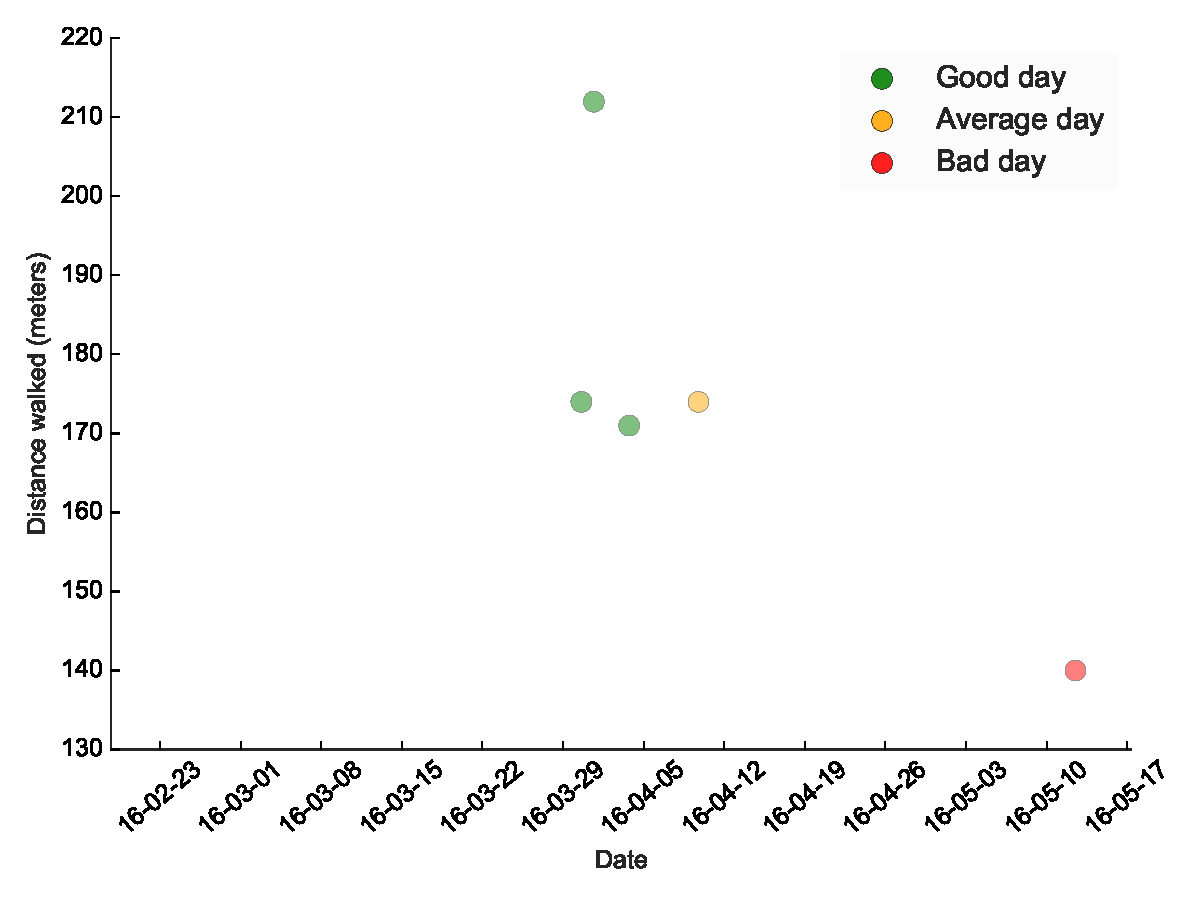
\includegraphics[scale=0.29]{img/walking/2Dy2uFf3aw6jv9r5u}
		\label{fig:user1}
	}
	\hspace{0.5cm}
	\subfloat[]{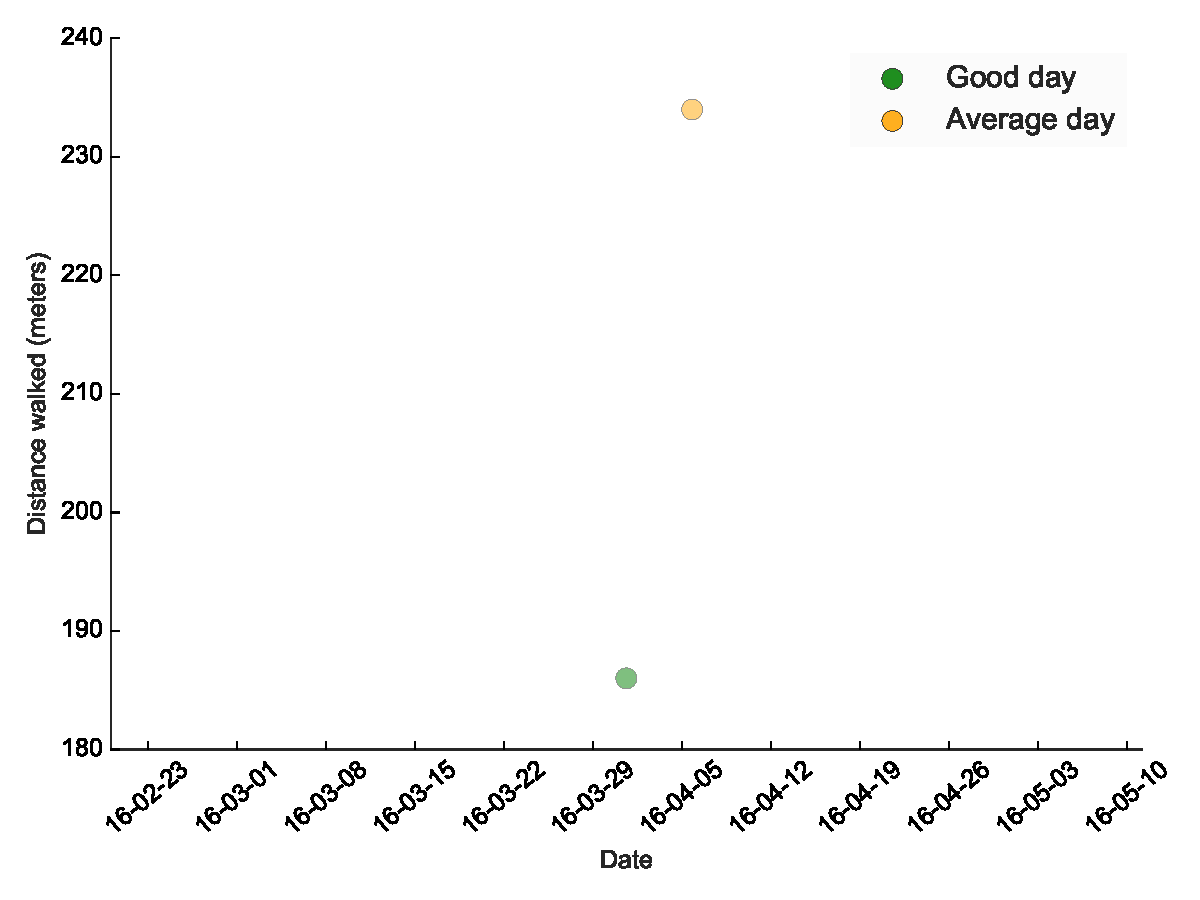
\includegraphics[scale=0.29]{img/walking/dW4YzJQEaidmyhsuY}
		\label{fig:user2}
	}
	\vfill
	\subfloat[]{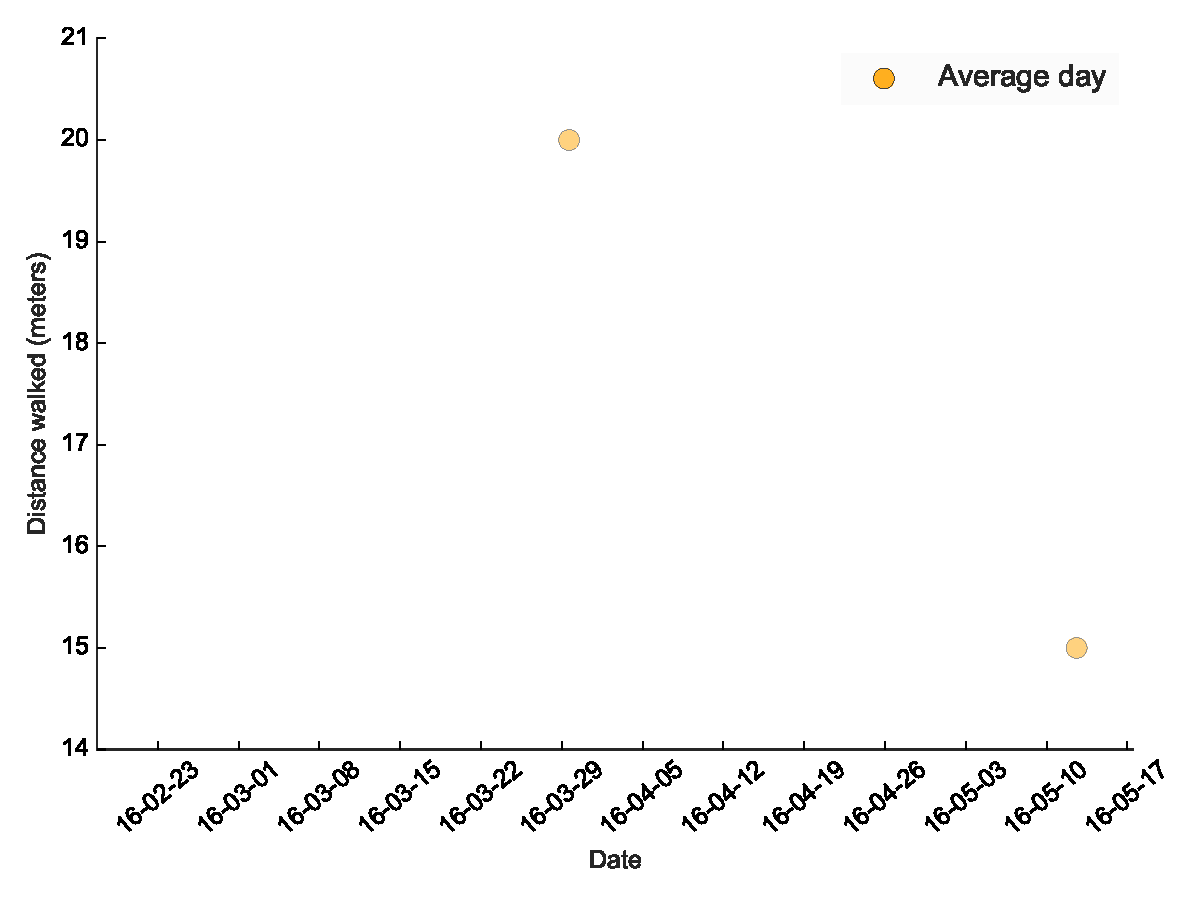
\includegraphics[scale=0.29]{img/walking/gGSWzh5PnqgFdCpq4}
		\label{fig:user3}
	}
	\hspace{0.5cm}
	\subfloat[]{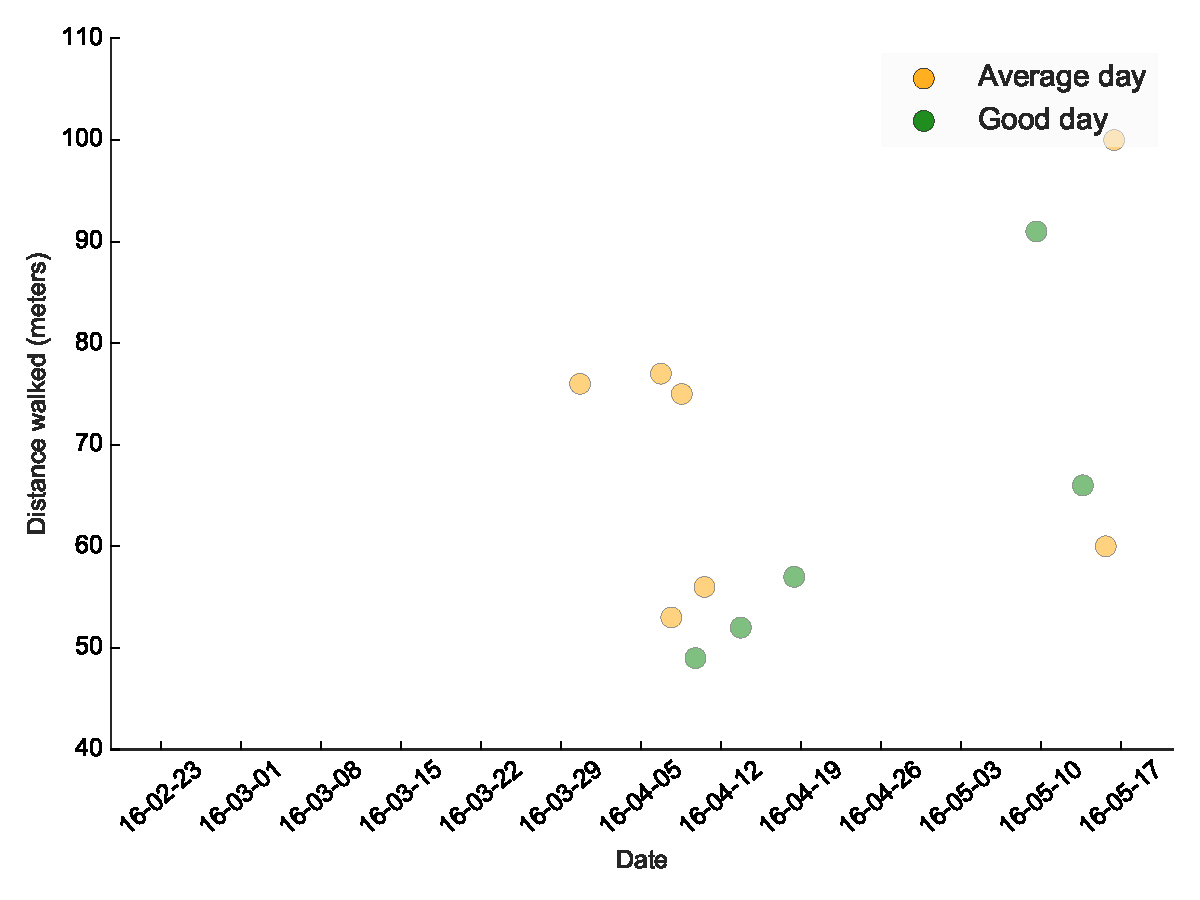
\includegraphics[scale=0.29]{img/walking/oGTtb7DQu4ewMBinx}
		\label{fig:user4}
	}
	\captionof{figure}{Plots of the walking durations of the participants. 
		Only dates that both had a rating and a measurement of distance walked are shown. 
		As can be seen in the legend of each of the figures, each point is colored according to the rating given by the participant for that specific day.}
	\label{fig:Walking Test Visualization}
\end{figure}
\newpage
%
To interpret the rest of the coefficients, we must look at the outcome of the correlation coefficient.
%
\begin{itemize}
	\item A positive correlation coefficient means that the ranks of both the variables are increasing.
	\item A negative correlation coefficient means that if the rank of one variable increases, the rank of the other variable decreases. 
	\item If both variables are independent, a coefficient with a value of zero would be expected.
\end{itemize}
%
For the other participants (\subref{fig:user1} and \subref{fig:user4}), the amount of samples is better.
For all of the coefficients, the corresponding $p$-value is never lower than $0.05$.
Therefore, there is no sign of statistical significance for each of the coefficients.
This lack of statistical significance makes it useless to try to interpret the correlation coefficients.
In the end, it seems like the amount of experiments for most of the participants is just too low to get meaningful results using statistical analysis.